% minimal setup for Debian Lenny:
% texlive-xetex
% texlive-lang-polish
% texlive-latex-recommended (xkeyval.sty)
% Junicode (Junius-Unicode) 
% Adobe Reader 8 nie odświeża!!!

% KPBC:
% http://kpbc.umk.pl/dlibra?action=ChangeLanguageAction&language=pl
% http://kpbc.umk.pl/dlibra/publication?id=17781
% http://kpbc.umk.pl/dlibra/docmetadata?id=34034

% http://fleksem.klf.uw.edu.pl/~jsbien/poufne/NKPoDjVu/iNKPo.djvu
% http://www.fileformat.info/info/unicode/font/index.htm

\documentclass[pdfpagemode=UseNone]{beamer}
\setbeamercovered{highly dynamic}
\usetheme{JuanLesPins}

%\documentclass{article}
% loaded anyway by xltxtra:
%\usepackage{fontspec} 

% backwards compatibility for accents:
% loaded anyway by xltxtra:
%\usepackage{xunicode}

% without this package CM fonts used by default:
\usepackage{xltxtra}
% why it doesn't work?
\defaultfontfeatures{Mapping=tex-text}

%\usepackage{polski}

\usepackage{hyperref}

\usepackage{longtable}

\usepackage{relsize}

% \usepackage[polish]{varioref}
% \renewcommand\reftextfaraway[1]{na str.~\pageref{#1}}
% \def\eob{ę}
% \def\aob{ą}



% loaded anyway by xltxtra:
% \usepackage{graphicx}


%\setmainfont[Mapping=tex-text]{Junicode}
\setmonofont{DejaVu Sans Mono}
% \font\Junicode="Junicode"
% \font\Mono="DejaVu Sans Mono"
% \Junicode

% Wilk
\usepackage{graphicx}
\usepackage{xcolor}
\newcommand\raw[1]{\colorbox{black!15}{\texttt{#1}}}
%\font\JunicodePolish="Junicode:mapping=DisplayOldPolish"
%\font\JunicodePolish="[/repliki/fleksem/Junicode/Junicode-Regular-JSB]"
\font\JunicodePolish="Junicode-Regular"
\font\Monofont="DejaVu Sans Mono"
\font\DejaVuSerif="DejaVu Serif"
\newcommand\stpl[1]{{\JunicodePolish\colorbox{black!15}{#1}}}
\newcommand\Emacs[1]{{\Monofont\colorbox{black!15}{#1}}}
\newcommand\mufi[1]{{\JunicodePolish\colorbox{green!15}{#1}}}
\newcommand\jsb[1]{{\JunicodePolish\colorbox{blue!15}{#1}}}
\newcommand\ucs[1]{{\JunicodePolish\colorbox{white!15}{\strut#1}}}

% ɑ -> 
\catcode`\ɑ=13
\defɑ{}

%  F1D6 LEFT LOWER SLANTED STROKE
\newcommand\alfac{}
\newcommand\ecaud{}
\newcommand\vcaud{}
% COMBINING LATIN SMALL LETTER E
\newcommand\eou{uͤ}

\let\mykeys\raw
\let\textel\raw
\let\KOMBIkeys\texttt
\let\Uname\texttt
\let\Ublock\texttt
\let\quotedfont\texttt
%\let\im\texttt
\newcommand\im[1]{\texttt{#1}}
\let\Fname\texttt
%\let\termin\textit
\newcommand\term[1]{\texttt{#1}}

\author{Janusz S. Bień}

\title{Historical Polish texts\\
and\\
Unicode\\(a case study --- work in progress)}
\date[2017]{\today}
%\date[2011]{????}

\begin{document}

\maketitle{}

\section{Preliminaries}
\label{sec:preliminaries}

 \begin{frame}
  \frametitle{Version Control System information}
% Needs Auctex at least 11.88:
\begin{center}

  Mercurial repository:

  \url{https://bitbucket.org/jsbien/Unicode4Polish}

  \bigskip
  
  Changeset and local revision:

\input{"| hg log -v -l 1 \jobname.tex --template '{node}'"}

\input{"| hg log -v -l 1 \jobname.tex --template '{rev}'"}

\end{center}
 \end{frame}

\begin{frame}
  \frametitle{Earlier work}
  \Large
  \begin{itemize}
  \item \url{http://bc.klf.uw.edu.pl/271/}
  \item \url{http://bc.klf.uw.edu.pl/179/}
  \item PDF available on request
  \item source files available on request 
  \end{itemize}
\end{frame}

\begin{frame}
  \frametitle{Three perspectives}

  \begin{block}{Focus temporarily on characters}
    \begin{itemize}
    \item Glyphs (fonts, OCR)
    \item Characters (coding and searching)
    \item Textels\\
      \url{http://bc.klf.uw.edu.pl/118/}
    \end{itemize}
  \end{block}
\end{frame}

\begin{frame}
  \frametitle{Unicode}

  Is sufficient without PUA?

  \begin{block}{Unicode Private Use Area}
      \begin{itemize}
      \item ConScript Unicode Registry\\
        (\url{http://www.evertype.com/standards/csur/})
      \item SIL (Summer Institute of Linguistics)\\
        (\url{http://scripts.sil.org/pua_home})
      \end{itemize}
    \end{block}
% To: Petr Tomasek <tomasek@etf.cuni.cz>
% Cc: Doug Ewell <doug@ewellic.org>,  Unicode Mailing List <unicode@unicode.org>
% Subject: Re: preparing a PUA specification (for historical Polish text)
% From: jsbien@uw.edu.pl
% --text follows this line--
% Petr Tomasek <tomasek@etf.cuni.cz> writes:

% >> 
% >> If you do want PUA assignments, it might be most appropriate to propose 
% >> these for inclusion in MUFI.
% >
% > Just curious: why MUFI and not SIL?
% > http://scripts.sil.org/pua_home
        \begin{block}{Medieval Unicode Font Initiative
        (\url{www.mufi.info})}
% http://www.hit.uib.no/mufi/PUAcoord/PUA-4.0-a-2.html
      \begin{itemize}
      \item MUFI character recommendation (version 3.0, 24 June 2009)
      \item Proposals for new MUFI characters 
      \end{itemize}
        \end{block}
\end{frame}

\begin{frame}
 \frametitle{Text Encoding Initiative}
 \begin{itemize}
 \item ENRICH's Gaiji Bank of non-standard
        characters and glyphs\\
        (\url{http://beta.manuscriptorium.com/index.php?q=node/3})
      \item \url{http://slovo-aso.cl.bas.bg/howto.html}
      \item \ldots
 \end{itemize}
\end{frame}

\begin{frame}
  \frametitle{Unicode and Polish language}
    \begin{block}{Sebastian Kembgen}
      \begin{itemize}
      \item Unicode 4.1 and Slavic Philology
  Problems and Perspectives (I)
      \url{http://kodeks.uni-bamberg.de/slavling/downloads/SK_Slavic_Unicode_I.pdf}
    \item  Unicode 4.1 and Slavic Philology
  Problems and Perspectives (II)
       \url{http://kodeks.uni-bamberg.de/slavling/downloads/SK_Slavic_Unicode_II.pdf}
      \end{itemize}
    \end{block}

\end{frame}



\section{Encoding and transcription}


\begin{frame}
  \frametitle{Scientific (diplomatic) transcription}
  \begin{block}{Theory}
    \begin{itemize}
    \item A book \textit{Principles of editing Old Polish texts}, 1955\\
      \url{http://ebuw.uw.edu.pl/publication/1334}:\\
      not sufficient for our purposes,\\ partly obsoleted by publishing technology
    \end{itemize}
  \end{block}
  \begin{block}{Practice}
    \begin{itemize}
    \item Dictionary of 16th century Polish:\\editor instruction and actual usage
    \end{itemize}
  \end{block}
  \begin{quote}
    In theory, practice is compatible with theory;\\
    in practice, it is not.\\
    (author unknown)
  \end{quote}
\end{frame}
\begin{frame}
  \frametitle{Scientific (diplomatic) transcription}
  \begin{block}{More theory}
    Krzysztof Opaliński\\
    Problemy kodowania korpusów historycznych\\
    (na przykładzie tekstów XVI-wiecznych)

    \bigskip
    Joanna Kamper-Warejko, Iwona Kaproń-Charzyńska (eds.)\\
    \textit{Z zagadnień leksykologii i leksykografii języków słowiańskich}\\
    Wydawnictwo Naukowe Uniwersytetu Mikołaja Kopernika\\
    Toruń 2007\\
    pages 107--114

  \end{block}
\end{frame}

\section{Case study}
\label{sec:case-study}
\begin{frame}
  \frametitle{Zasady}
  
\includegraphics[width=\hsize]{img/Zasady-tyt}
\end{frame}

\begin{frame}
  \frametitle{Autorzy}
  \begin{enumerate}
  \item Konrad Górski, zm. 7 kwietnia 1990 w Toruniu
  \item Władysław Kuraszkiewicz, zm. 10 marca 1997 w Poznaniu
  \item Franciszek Pepłowski, zm. 2009\\
    {\relsize{-2}\url{http://www.linguistica.umk.pl/teksty/02_kaminska.pdf}}
  \item Stefan Saski, zm. 1974\\
    {\relsize{-2}\url{http://www.archpan.poznan.pl/wp-content/uploads/2015/11/Materia\%C5\%82y-Stefana-Saskiego-P-III-62.pdf}}
\item Witold Taszycki, zm. 9 sierpnia 1979 w Krakowie
\item Stanisław Urbanczyk, zm. 23 października 2001 w Krakowie
\item Stefan [Vrtel-]Wierczynski, zm. 3 lutego 1963 w Poznaniu 
\item Jerzy Woronczak, zm. 6 marca 2003 we Wrocławiu
  \end{enumerate}
\end{frame}

\begin{frame}
  \frametitle{Utwór wspólny (nie zbiorowy)}
W R O C Ł A W 1955\\
ZAKŁAD IMIENIA OSSOLINSKICH\\
WYDAWNICTWO POLSKIE] AKADEMII NAUK

\bigskip
Redacja naukowa\\
MARIA RENATA MAYENOWA\\
przy współudziale\\
ZOFII FLORCZAK\\

\end{frame}

\begin{frame}
  \frametitle{Zasady s. 27 w. 30}
  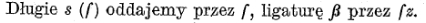
\includegraphics[width=\hsize]{img/Zasady27-30}

  OCR:\\
  \begin{quote}
  \texttt{Długie s ([ ) oddajemy przez [ , ligaturę [3 przez [z.}
\end{quote}

  {\stpl{ſ}}
    \texttt{LATIN SMALL LETTER LONG S}

    {\stpl{ß}}
    \texttt{LATIN SMALL LETTER SHARP S}

    \url{https://en.wikipedia.org/wiki/ß}
    \url{https://pl.wikipedia.org/wiki/ß}

    \begin{block}{Komentarze}
      Dlaczego \textit{ſz}?

      PESEL, \ldots

      \stpl{ẞ} \texttt{LATIN CAPITAL LETTER SHARP S}
    \end{block}
    
\end{frame}

\begin{frame}
  \frametitle{Zasady s. 27 w. 31-34}
  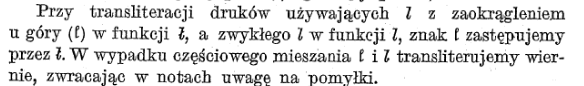
\includegraphics[width=\hsize]{img/Zasady27-31_34}

  OCR:
  \begin{quote}
Przy transliteracji druków używajacych Z z zaokragleniem
u góry ( f) w funkcji ł, a zwykłego Z w funkcji Z, znak li zastępujemy
przez t. W wypadku częściowego mieszania E i Z transliterujemy wier-
nie, zwracajac w notach uWagę na pomyłki.
\end{quote}
\end{frame}


\begin{frame}
  \frametitle{Zasady s. 27 w. 31-34}

  \url{https://en.wikipedia.org/wiki/Ł}
  \url{https://pl.wikipedia.org/wiki/Ł}
  
  \begin{block}{Komentarze}
      Nie tylko traktat Parkosza?

      Podobny wygląd:\\
      
      {ℓ} \texttt{SCRIPT SMALL L}

      {𝓁} \texttt{MATHEMATICAL SCRIPT SMALL L}
      
    \end{block}
\end{frame}



\end{document}
echo -n -e "$(echo http://ru.wikipedia.org/wiki/xxx | sed 's/+/ /g;s/%\(..\)/\\x\1/g;')"

https://en.wikipedia.org/wiki/Ł

ą ℓ {\displaystyle \ell } \ell ,

 2113
MATHEMATICAL SCRIPT SMALL L U+1D4C1 

%%% Local Variables: 
%%% coding: utf-8-unix
%%% mode: latex
%%% TeX-PDF-mode: t
%%% TeX-engine: xetex
%%% TeX-master: t
%%% TeX-command-extra-options: "-shell-escape"
%%% End: 
